\documentclass{beamer}
%21.39
%21.52
%22.07
%% Use package -----------------------------------------------------------------

\usepackage[T1]{fontenc}
\usepackage[utf8]{inputenc}
\usepackage{lmodern}
\usepackage{graphicx}
\usepackage[absolute,overlay]{textpos}
\usepackage{multicol}
\usepackage{listings}

\usepackage{multimedia}

\usepackage{svg}




%% Beamer customization---------------------------------------------------------

\usepackage{xcolor}
\usetheme{Warsaw}

%% Themes
% Outer themes
\useoutertheme{shadow}
% Rounded boxes and shadows
\useinnertheme[shadow=true]{rounded}
% Solid \item symbols
\useinnertheme{circles}

%% Custom colors
\definecolor{rltgreen}{rgb}{0,0.5,0}
\definecolor{pasteur}{RGB}{0,90,154}
\setbeamerfont{block title}{size={}}
\setbeamercolor{structure}{fg=pasteur}
\setbeamercolor{item}{fg=pasteur}

%Color of title
\setbeamertemplate{frametitle}
{
    \nointerlineskip
    \begin{beamercolorbox}[sep=0.3cm,ht=1.8em,wd=\paperwidth]{frametitle}
        \vbox{}\vskip-2ex%
        \strut\insertframetitle\strut
        \vskip-0.8ex%
    \end{beamercolorbox}
}
% Hide navigation symbols
\setbeamertemplate{navigation symbols}{}

%% Title block
\setbeamercolor*{title}{use=structure,fg=white,bg=pasteur}

%% Bottom infolines
\setbeamertemplate{footline}
{
  \leavevmode%
  \hbox{%
  \begin{beamercolorbox}[wd=.3\paperwidth,ht=2.25ex,dp=1ex,center]{author in head/foot}%
    \usebeamerfont{author in head/foot}\insertshortauthor
  \end{beamercolorbox}%
  \begin{beamercolorbox}[wd=.7\paperwidth,ht=2.25ex,dp=1ex,center]{title in head/foot}%
    \usebeamerfont{title in head/foot}\insertshorttitle\hspace*{3em}
    \insertframenumber{} / \inserttotalframenumber\hspace*{1ex}
  \end{beamercolorbox}}%
  \vskip0pt%
}
\makeatletter

%% Top infolines
\setbeamertemplate{headline}{%
\leavevmode%
  \hbox{%
    \begin{beamercolorbox}[wd=\paperwidth,ht=2.5ex,dp=1.125ex]{palette quaternary}%
    \insertsectionnavigationhorizontal{\paperwidth}{}{\hskip0pt plus1filll}
    \end{beamercolorbox}%
  }
}

%% Define Snakemake ------------------------------------------------------------

\definecolor{eclipseBlue}{RGB}{42,0.0,255}
\definecolor{eclipseGreen}{RGB}{63,127,95}
\definecolor{eclipsePurple}{RGB}{127,0,85}

\lstset{language=Python}
\lstset{
    basicstyle=\tiny\ttfamily,
    morekeywords={rule, output, shell, params, run, configfile, temp, threads, log},
    showstringspaces=false,
    commentstyle=\color{eclipseGreen}, % style of comments
    keywordstyle=\color{eclipsePurple}, % style of keywords
    stringstyle=\color{eclipseBlue}, % style of strings
}


%% Set up title ----------------------------------------------------------------

\title{ Snakemake (single cell) integration in Sequana}
\author[T.Cokelaer]{Thomas Cokelaer}
\institute{Institut Pasteur}
\date{Nov 9th 2017\\}

\begin{document}

%% Title slide -----------------------------------------------------------------

\begin{frame}[plain]
    \titlepage
    \begin{textblock*}{5cm}(4.5cm,0.3cm)
        \includegraphics[scale=0.09]{images/Institut_Pasteur.png}
    \end{textblock*}
\end{frame}



%---------------------------------------------------------------------

\section{Snakemake}

\begin{frame}[plain]
 \centering
 \begin{Huge}
 Snakemake: a workflow manager
 \end{Huge}
\end{frame}



\begin{frame}
\frametitle{Many bioinformatic pipeline frameworks available}
\centering
 \begin{figure}
 \includegraphics[scale=0.23]{images/workflows.png}
 \end{figure}
 A review of bioinformatic pipeline frameworks. Jeremy Leipzig
Briefings in Bioinformatics, Volume 18, Issue 3, 1 May 2017, Pages 530–536, 
https://doi.org/10.1093/bib/bbw020

 \end{frame}


\begin{frame}
\frametitle{Many bioinformatic pipeline frameworks available}
\centering
 \begin{figure}
 \includegraphics[scale=0.4]{images/cloud.png}
 \caption{word cloud of 103 
frameworks' description (less 
framework / pipeline / worfflow) https://github.com/pditommaso/awesome-pipeline}
 \end{figure}
 \end{frame}


\begin{frame}
 \frametitle{Which framework to choose ?}
 
 There are many frameworks out there. \\
 \vspace{.5cm}
 \pause 
 Some are \textbf{professional}, others not. \\
 \vspace{.5cm}
 \pause 
 Some are not \textbf{maintained} anymore or by a few developers. \\
 \vspace{.5cm}
 \pause 
 Many frameworks pass those filters. We have the luxury to 
choose one amongst many good frameworks !
 \\
 \vspace{.5cm}
 So you need to define your 
requirements in terms of portability, language, reproducibility, 
parallelization, etc ? 
\end{frame}
 
 
 \begin{frame}
  \frametitle{Which framework to choose ?}
  \begin{itemize}
   \item We need to be reactive
   \item Those days, developers code in R or Python. 
   \item We need (non intrusive) parallelization in the NGS field
  \end{itemize}
  
\begin{alertblock}{}
 What about Snakemake ?
\end{alertblock}
  
  
 \end{frame}

 

\begin{frame}[plain]
\centering
 \begin{overprint}
    \onslide<1>\includegraphics[scale=0.3]{./images/equation2.png}
    \onslide<2>\includegraphics[scale=0.3]{./images/equation1.png}
\end{overprint}
\end{frame}


\begin{frame}
\frametitle{Think Makefile, think DAG}
    
   \centering \textbf{Snakemake is a workflow manager}\\
      
        \only<1> 
        {
            \begin{figure}
                \includegraphics[width=\textwidth,height=0.6\textheight]{images/dag_0.png}
                \caption[1]{A \textit{pipeline} problem}
            \end{figure}                
        }
        \only<2> 
        {
            \begin{figure}
                \includegraphics[width=\textwidth,height=0.6\textheight]{images/dag_1.png}
                \caption[1]{Ideal for embarassingly parallel problem}
            \end{figure}                
        }\only<3> 
        {
            \begin{figure}
                \includegraphics[width=\textwidth,height=0.6\textheight]{images/dag_2.png}
                \caption[1]{Ideal for embarassingly parallel problem}
            \end{figure}                
        }
        \only<4> 
        {
            \begin{figure}
                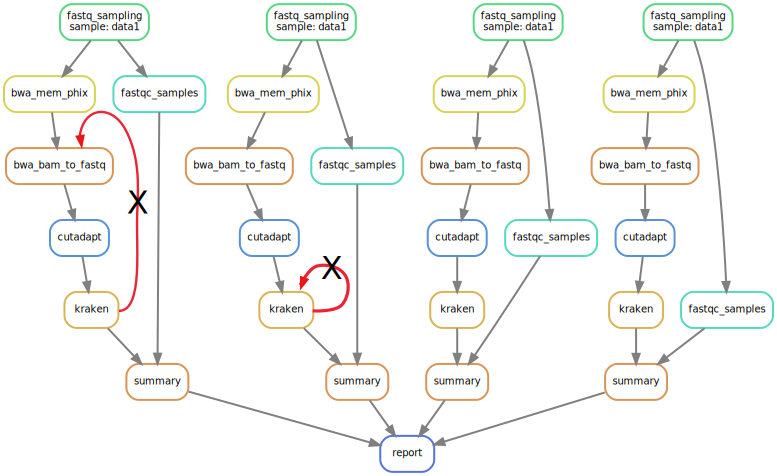
\includegraphics[width=\textwidth,height=0.6\textheight]{images/dag_wrong2.png}
                \caption[2]{Requires a DAG (no self loop of feedback loop allowed !)}
            \end{figure}
        }
  % Snakemake c'est plus que M + P
  % C'est aussi un workflow manager qui est PRATIQUE. 
  %Par forcement facile mais PRATIQUE.
\end{frame}




% ------------------------------------------------------


\begin{frame}
\frametitle{The problem}
Let us consider two FastQ files (independent samples) and let us map them on a reference (phiX174). The two 
sample files are named sample\_A.fastq.gz and sample\_B.fastq.gz
  \begin{figure}
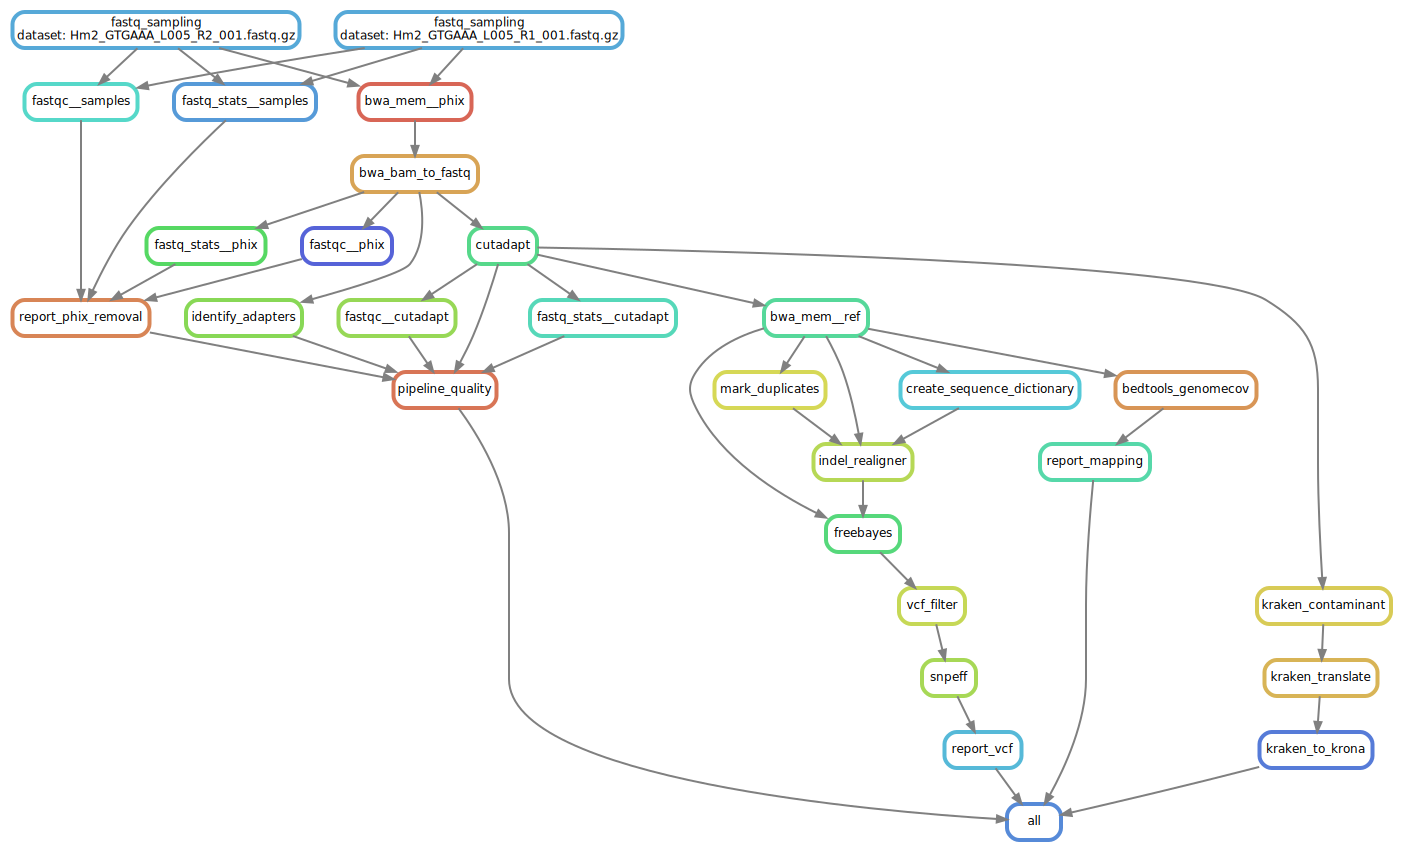
\includegraphics[width=0.5\textwidth, height=0.5\textheight]{images/dag.png}
  \end{figure}
\end{frame}



% --------------------------------------------------------------------------

\begin{frame}[fragile]
    \frametitle{Snakefile example}
    
    \begin{block}{Snakefile}
    \begin{lstlisting}
SAMPLES = ["sample_A", "sample_B"]

rule all:
    input: expand("mapped_sample/{sample}.bam", sample=SAMPLES)

rule bwa_index:
    input: "phiX174.fa"
    output: "phiX174.fa.bwt"
    shell: "bwa index {input}"

rule bwa_mapping:
    input:
        ref = "phiX174.fa",
        index = "phiX174.fa.bwt",
        fastq = "{sample}.fastq.gz"
    output: "mapped_sample/{sample}.bam"
    shell:
        "bwa mem {input.ref} {input.fastq} | samtools view -Sb - > {output}"
    \end{lstlisting}
    \end{block}
\end{frame}



\begin{frame}[fragile]
\frametitle{Execution}

      \begin{block}{In a shell, type:}
	  \begin{lstlisting}[basicstyle=\large]
	  snakemake -s gc_minimalist.rules 
	  \end{lstlisting}
      \end{block}
    \begin{block}{Stdout}
    \centering
    \includegraphics[scale=0.3]{images/screen1.png}
    \end{block}     
    
    
More options if a configuration file is required, or execution is on a cluster, 
or \dots something goes wrong.
\end{frame}


         
        
% ----------------------------------------------

\begin{frame}[fragile]
    \frametitle{Config file}
     We can use a configuration file for parameters. Format are either JSON or YAML
    The community seems to prefer YAML.
    
    \begin{block}{config.yaml}
        \begin{lstlisting}
samples: [DOLPHINS, WHALES]
windows: [512,1024,2048,4096]
        \end{lstlisting}
    \end{block}
    \begin{block}{Snakefile}
    \begin{lstlisting}
configfile: "config.yaml"

rule all:
    input: expand("{dataset}_{ws}.png", 
                          dataset=config['samples'], 
                          ws=config['windows'])

rule spectrogram:
    input:  "{dataset}.wav"
    output: "{dataset}_{window}.png"    
    shell:  "python spec.py {input} {wildcards.window}"
    \end{lstlisting}
    \end{block}
\end{frame}


% -------------------------------------------------------------



\begin{frame}[fragile]
\frametitle{Cluster execution}

No intrusive code. It just worked on SGE and then on a SLURM cluster 
without changing a single line of code !

\begin{lstlisting}
# execute the workflow on cluster with qsub submission command
# (and up to 100 parallel jobs)
snakemake --cluster qsub --jobs 100

# tell the cluster system about the used threads
snakemake --cluster "qsub -pe threaded {threads}" --jobs 100

# execute the workflow with DRMAA
snakemake --drmaa --jobs 100

# execute the workflow on cluster with sbatch (SLURM)
snakemake --cluster "sbatch --qos fast" --jobs 100

\end{lstlisting}
\end{frame}


\begin{frame}[plain]
 \centering
 \begin{Huge}
 Sequana
 \end{Huge}
\end{frame}



\begin{frame}
\frametitle{Motivation}
\begin{block}{Jan 2015: provide NGS pipelines to Biomics sequencing platform 
https://research.pasteur.fr/en/team/biomics/ (Institut Pasteur)}
 \begin{itemize}
  \item Genomics: QC + variant calling + de-novo
  \item Transcriptomics: RNA-seq + ChIP-seq 
  \item Metagenomics
  \item Illumina but also Pacbio long reads technologies
 \end{itemize}
 %\includegraphics{images/genetic_strand.png}
 %\includegraphics{images/strand.png}
\end{block} 
\end{frame}


\begin{frame}
\frametitle{How ?}

\begin{columns}
\begin{column}{1.5cm}
\includegraphics[height=0.2\textheight]{images/logo_python.png} 
\end{column}
\begin{column}{9cm}
a glue language, a scientific language
\end{column}
\end{columns}


\rule{\textwidth}{1pt}


\begin{columns}
\begin{column}{1.5cm}
\includegraphics[height=0.2\textheight]{images/logo_snakemake.png}
\end{column}
\begin{column}{9cm}
a pipeline 
framework mixing Python and Makefile \\
{\footnotesize \textcolor{blue}{\textit{Köster, Johannes and Rahmann, Sven. 
Snakemake - A scalable 
bioinformatics workflow engine. Bioinformatics 2012.}}}
\end{column}
\end{columns}

\rule{\textwidth}{1pt}


\begin{columns}
\begin{column}{1.5cm}
\includegraphics[height=0.2\textheight]{images/exe.png}
\end{column}
\begin{column}{9cm}
Dedicated standalone such as genome coverage characterisation or a graphical 
user interface for Snakemake pipelines (Sequanix).
%{\footnotesize \textcolor{blue}{\textit{D. Desvillechabrol, C. 
%Bouchier, S. Kennedy, T. Cokelaer Detection and characterization of low 
%and high genome coverage regions .... BioRxiv 
%https://doi.org/10.1101/092478 }}. Submitted to GigaScience journal }
\end{column}
\end{columns}



\end{frame}




\section{Sequana pipelines (an overview)}


\begin{frame}
\frametitle{Pipeline example: quality control pipeline} 
\centering
\includegraphics[height=0.8\textheight, width=\textwidth]{./images/dag2.png}
\end{frame}



\begin{frame}
\frametitle{Pipeline example: variant calling} 
\centering
\includegraphics[height=0.8\textheight, 
width=\textwidth]{./images/variant_calling_dag.png}
\end{frame}


\begin{frame}{Pipeline complexity}
    \includegraphics[width=11cm, height=7cm]{images/number_of_rules.png}
\end{frame}


\begin{frame}{Factorization}
\centering
    \includegraphics[width=8cm]{images/rules_reusing.png}
\end{frame}




\section{Sequanix}

\begin{frame}[plain]
 \centering
 \begin{Huge}
 Sequanix
 \end{Huge}
\end{frame}

\begin{frame}{GUI to simplify the usage of snakemake}
    \begin{columns}
        \begin{column}{0.5\textwidth}

            \only<1>{\includegraphics[scale=0.25]{../../images/sequana_init}}

            \only<2>{\includegraphics[scale=0.25]{../../images/choose_pipeline}}

            \only<3>{\includegraphics[scale=0.25]{../../images/choose_input_output}}

            \only<4>{\includegraphics[scale=0.25]{../../images/sequana_pipeline}}

            \only<5>{\includegraphics[scale=0.25]{../../images/sequana_running}}

            \only<6>{\includegraphics[scale=0.25]{../../images/sequana_finish}}

        \end{column}
        \begin{column}{0.5\textwidth}
            \only<1>{
                \begin{itemize}
                    \item Interface developed with PyQT5 and python
                    \item Wrap our snakemake pipelines to ease the usage
                    \item Usable on our cluster, which allows X11
                \end{itemize}
            }
            \only<2-6>{
            \begin{enumerate}
                \item<2-6> Choose a pipeline
                \item<3-6> Set input and output
                \item<4-6> Fill the config formular
                \item<5-6> Run the pipeline
                \item<6> Finished !
            \end{enumerate}
            }
        \end{column}
    \end{columns}
\end{frame}




\section{Sequana: Continuous integration}
\input{../../slides/slide_sequana_ci_2017_oct}




\section{pipeline integration}

\begin{frame}[plain]
 \centering
 \begin{Huge}
 Third party pipeline integration
 \end{Huge}
\end{frame}


\begin{frame}
\frametitle{Solution 1: the easiest}
Using sequanix: manual import of the pipeline and click run.
\end{frame}

\begin{frame}
\frametitle{Solution 2: the collaborative and robust one}
\begin{block}{Needs}
 \begin{itemize}
  \item versioning
  \item collaborative
  \item visibility
  \item testing
  \item flexibility (how to change a rule)
 \end{itemize}
\end{block}

\begin{block}{Solutions}
 \begin{itemize}

\item integrate within a github repository
 \item use git to acknowledge contributions
 \item use online documentation
 \item testing of use-case scenario (TODO)
 \item Use snakemake rules, define several pipelines taylored for each group if 
needed.
 \end{itemize}
\end{block}
Using sequanix: sequana import of the pipeline and click run.
\end{frame}


\begin{frame}
 \frametitle{Where to go ?}
 \begin{itemize}
  \item Integrate the mars-seq QC pipeline in a common repo. It could be 
an existing sequana repository. 
  \item Provide a test-case scenario for testing
  \item Test and validate integration of mars-seq snakemake pipeline inside 
Sequanix.
 \end{itemize}

\end{frame}


\end{document}
